\chapter{Exploration of Chemical Space}
%
\section{Introduction}
%
In order to jump from one chemical state to another, we must be able to propose a chemical state to visit. In the language of the Metropolis~\cite{Hastings1970} algorithm, I will denote this proposal density $q(\cdot~|~k)$.
%
For the purpose of the correctness of this algorithm, the formal requirements that I will place on $q(\cdot | k)$ are:
\begin{itemize}
    \item The proposal must be reversible: $q(k'|k) > 0 \Rightarrow q(k|k') >0$
    \item For every pair of states $k_0$ and $k_N$, $\exists \ \{k_0, ... ,k_N\} \ s.t. \ \prod\limits_{i=0}^{N-1} q(k_{i+1}|k_i) > 0$
\end{itemize}
%
The first condition implies reversibility: that is, if the algorithm can propose to jump forward, it can (possibly with a different probability) propose to jump backwards. The second condition implies that there are no states that are ultimately unreachable from any other state.
%
Although this seems straightforward, and many obvious choices are apparent, the quality of the proposal distribution has a profound impact on the performance of the algorithm~\cite{vanRavenzwaaij2018} and many adaptive techniques have been developed in other MCMC applications for this reason~\cite{Roberts2009}.
%
Not only does the proposal distribution need to satisfy the above basic requirements, it also must propose states to which a transition is feasible (in simulation terms) as well as provide the opportunity for far enough jumps that the simulation effectively explores chemical space. 
%
Feasibility in simulation terms has multiple aspects.
%
One such aspect is that the remainder of the algorithm (the dimension matching and the nonequilibrium switching, specifically) must be capable of completing the proposal.
%
Importantly, this involves how the atoms will be mapped between the current and proposed states.
%
Recall that the systems corresponding to chemical states $k$ and $k'$ do not typically have the same dimensionality.
%
However, it is a choice of the algorithm to choose which dimensions should be considered in common between the two endpoint systems, and which should be considered to be unique to the endpoints.
%
This choice--the atom mapping problem--will have a profound impact on the efficiency of the overall algorithm, as discussed below.
%
However, before concerning ourselves with the efficiency of the algorithm, the atom map must at least ensure that the proposal can be completed.
%
The requirement imposed by the dimension matching algorithm (discussed in Chapter~4) is that there must always be at least three atoms with positions (that is, either mapped or proposed by the dimension matching) forming a dihedral angle with each unique atom.
%
The nonequilibrium switching implementation requires that constraint lengths do not change.
%
In principle, this is not a formal requirement, but to avoid computing the necessary Jacobian, we do not map hydrogens, as typically only bonds to hydrogens are constrained.
%
To add to these challenges, in the terms of the simulation's operator, one would like to explore regions of chemical space that are feasible to purchase or synthesize as determined by models~\cite{Warr2014}, or otherwise avoid regions that are unfavorable for reasons besides binding free energy.
%
\section{Quantitative Metrics}
%
In principle, one might choose to base proposal probability from state $k$ to state $k'$ on the thermodynamic length of the path from $p(x, k)$ to $p(x', k')$. This quantity, described at length in \cite{Crooks2007, Sivak2012,Zulkowski2012}, is given by:
\begin{eqnarray}
\mathcal{L} &\equiv& \int_{0}^{1} dt \, \sqrt{\left.\dv{\lambda_i}{t}\right|_\lambda g_{ij}(\lambda) \left.\dv{ \lambda_j}{t} \right|_\lambda} \label{thermolength} \\
g_{ij} (\lambda) &\equiv& \mathrm{E} \left[ \pdv{\ln p(x)}{\lambda_i} \pdv{\ln p(x)}{\lambda_j} \right] = \int dx \, p(x) \, \pdv{\ln p(x)}{\lambda_i} \pdv{\ln p(x)}{\lambda_j} \label{metric_tensor}
\end{eqnarray}
%
where $\lambda(t)$ is a multidimensional control parameter that in this case interpolates between $p(x,k)$ for $t=0$ and $p(x', k')$ for $t=1$ along a predefined path. 
%
The quantity in Eq.~\ref{metric_tensor} is clearly the Fisher information metric; the quantity in Eq.~\ref{thermolength} is known as the thermodynamic length, and it captures a sense of how much work will be done by the transition attempt.
%
Importantly, the Cramer-Rao inequality reminds us that the variance of any unbiased estimator is lower-bounded by the inverse of the Fisher information~\cite{Rao1992}; to put this into terms relating to this work, the larger the differences between distributions in each step of the transition from $k$ to $k'$, the higher the lower bound on the variance of the acceptance probability.
%
It seems intuitive then that we would want to choose transition protocols that minimize this quantity; however, a quick inspection reveals that it is at least as difficult to compute as the relative free energy.
%
It thus seems impractical to propose states based on the thermodynamic length, since this is in practice very difficult to compute.
%
However, as an aside, it may be possible to learn this quantity from data.
%
Additionally, some other works have devised sophisticated approximate sampling algorithms to find near-optimal paths~\cite{Gingrich2016}.
%
Having completed many simulations, the thermodynamic length for each may be estimated, and fed to a machine learning model to predict thermodynamic lengths in future calculations.
%
Although this sounds appealing, it is important to note that the thermodynamic length depends not just on the identity of the chemical ligand, but also on its environment (for instance, a protein), which will vary depending on the calculation.
%
More work is required to explore this approach.
%
\section{Practical Approaches}
%
Despite the inherent difficulty in choosing chemical states as above, there exist several useful heuristic approaches to which we may resort.
%
Note that in the process of transitioning from one chemical species to another, we must identify which degrees of freedom belong to both systems, and which must be added or deleted.
%
We can use the number of degrees of freedom in common as a basis for the proposal distribution, under the assumption that the more degrees of freedom in common between the endpoint systems, the more likely the transition is to be accepted.
%
\subsection{Chemical State Proposal Algorithm}
%
In order to propose a chemical state $k'$ from a current state $k$, we first must derive the proposal probabilities.
%
Since atom mapping will be essential to the performance of the algorithm, we choose to use the number of atoms in an atom map as proportional to the proposal probability.
%
The atom maps themselves are derived from a maximum common substructure search~\cite{Englert2015} as implemented in the OpenEye toolkit.
%
This algorithm attempts to find the largest contiguous substructure that is present in both molecule graphs,
and has several hyperparameters that can be tuned or optimized.
%
More specifically, upon initialization, the proposal algorithm performs the following steps, given a set of molecules $\{ \mathcal{M}_0, \ldots, \mathcal{M}_N\}$ corresponding to chemical states $\{k_0, \ldots, k_N\}$:
% TODO: The $\{k_0, \ldots, k_n\}$ notation is super awkward. Why not just use $\{1, \ldots, K\}$?
%
\begin{itemize}
    \item For each pair of molecules $(\mathcal{M}_i, \mathcal{M}_j)$, perform a maximum common substructure search (MCSS)~\cite{Englert2015} to obtain a set of maps. In order to be valid, the map must contain at least three contiguous atoms, and must not map constrained bonds of different lengths.
    %
    \item Choose the mapping of atoms (that is, the list of which atoms should be considered degrees of freedom in common) with the maximum number of atoms.
    %\item Set unnormalized proposal probability $q_{ij} = q_{ji} = n_{atoms}$
    %
    %\item For each chemical pair of states $(i, j)$, $q(j~|~i) = \frac{h_{ij}}{\sum_{j=0}^{N} q_{ij}}$
    \item The probability of proposing $j$ given current state $i$, termed $q(j~|~i)$, is proportional to the number of atoms in common in the MCSS map.
    %
\end{itemize}
%
When running the simulation, the algorithm performs a proposal as follows:
\begin{itemize}
    \item Perceive the current chemical state of the simulation $k$
    \item Propose a state $k'$ from $q(\cdot~|~k)$
    \item Compute atom map and $\ln P_\mathrm{forward} = q(k'~|~k)$
    \item Compute $\ln P_\mathrm{reverse} = q(k~|~k')$
    %\item Return proposed state $k'$, atom map, and $(\ln P_\mathrm{reverse}-\ln P_\mathrm{forward})$
\end{itemize}
%
As described above, there are several hyperparameters here that can profoundly impact the performance of the algorithm. 
%
Foremost among them are the hyperparameters of the MCSS search: which atoms should we count as being in common?
%
Second, should the algorithm allow the creation and deletion of partial rings?
%
Although this would result in a larger atom map, it may be less favorable.
%
Third, the algorithm can optionally also sample from the list of atom maps, if there is more than one result.
%
Finally, the map produced must be usable by the following components of the algorithm.
%
\subsection{MCSS Hyperparameters}
%
When performing an MCSS search on chemical graphs, one must recognize that it is not simply the graph structure that is important, but also the labels on the edges and vertices, which correspond to bonds and atoms, respectively.
%
\begin{figure}
    \centering
    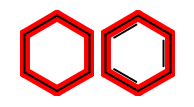
\includegraphics{benzene_cyclohexane_map.png}
    \caption{An example of an apparently reasonable atom map between benzene and cyclohexane.
    }
    \label{fig:benzene_cyclohexane_map}
\end{figure}
%
\begin{figure}
    \centering
    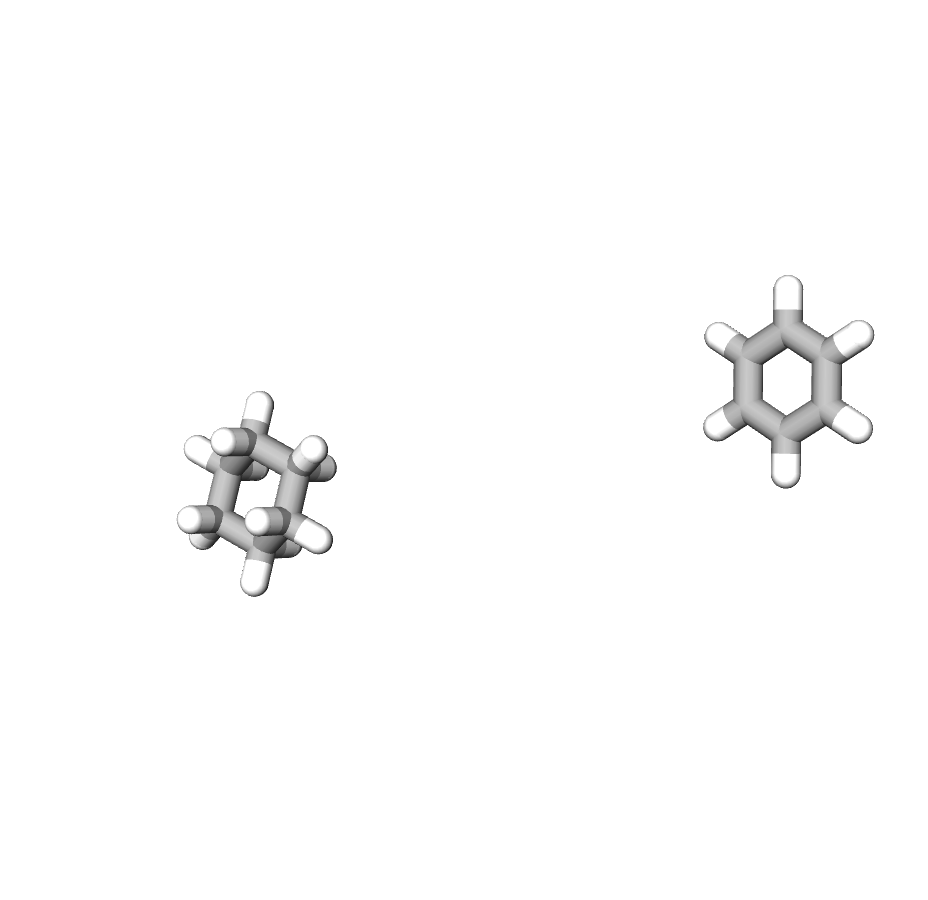
\includegraphics[width=1.0\textwidth]{cyclohex_ben_3d.png}
    \caption{3D structures of benzene and cyclohexane. Note that benzene is flat, while cyclohexane adopts a "chair" conformation.}
    \label{fig:benzene_cyclohexane_3D}
\end{figure}
%
To illustrate the consequence of improper atom maps (for instance, that disregard bond order), note Figure~\ref{fig:badbondorder}.
%
\begin{figure}
    \centering
    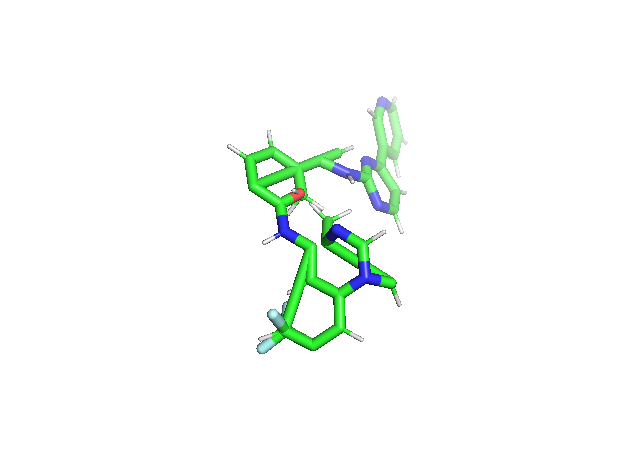
\includegraphics[width=1.0\textwidth]{failed_ring.png}
    \caption{A geometry that was constructed from an atom map that left no space to properly close the rings.}
    \label{fig:badbondorder}
\end{figure}
%
The simple inclusion of the bond order as a criterion for atom mapping greatly enhances the geometry that is produced, as in Figure~\ref{fig:goodbondorder}
%
\begin{figure}
    \centering
    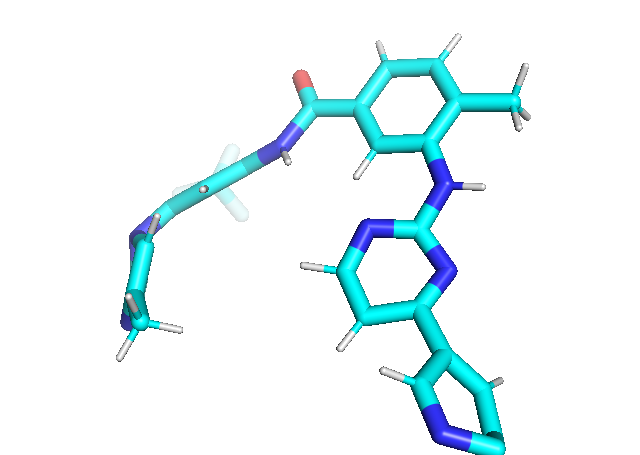
\includegraphics[width=1.0\textwidth]{success_ring_closure.png}
    \caption{A geometry resulting from the inclusion of bond order as a criterion for mapping atoms. More of the system is rebuilt, so a better geometry can be created.}
    \label{fig:goodbondorder}
\end{figure}
%
\section{Factors that affect acceptance probability}
%
For example, in Figure~\ref{fig:benzene_cyclohexane_map}, there are two molecules with six-membered carbon rings.
%
Mapping these would seem intuitive based on graph structure, but the nature of the edges makes this prohibitively unfavorable.
%
The 3D structures of these molecules, visualized in Figure~\ref{fig:benzene_cyclohexane_3D}, demonstrate that this is highly infeasible---the initial structure of either will be very unfavorable using the potential of the other.
%
In this case, chemical intuition would make the problem obvious: benzene is aromatic, while cyclohexane is not.
%
In many other cases, the distinction may not be clearly obvious.
%
\begin{figure}[h]
    \centering
    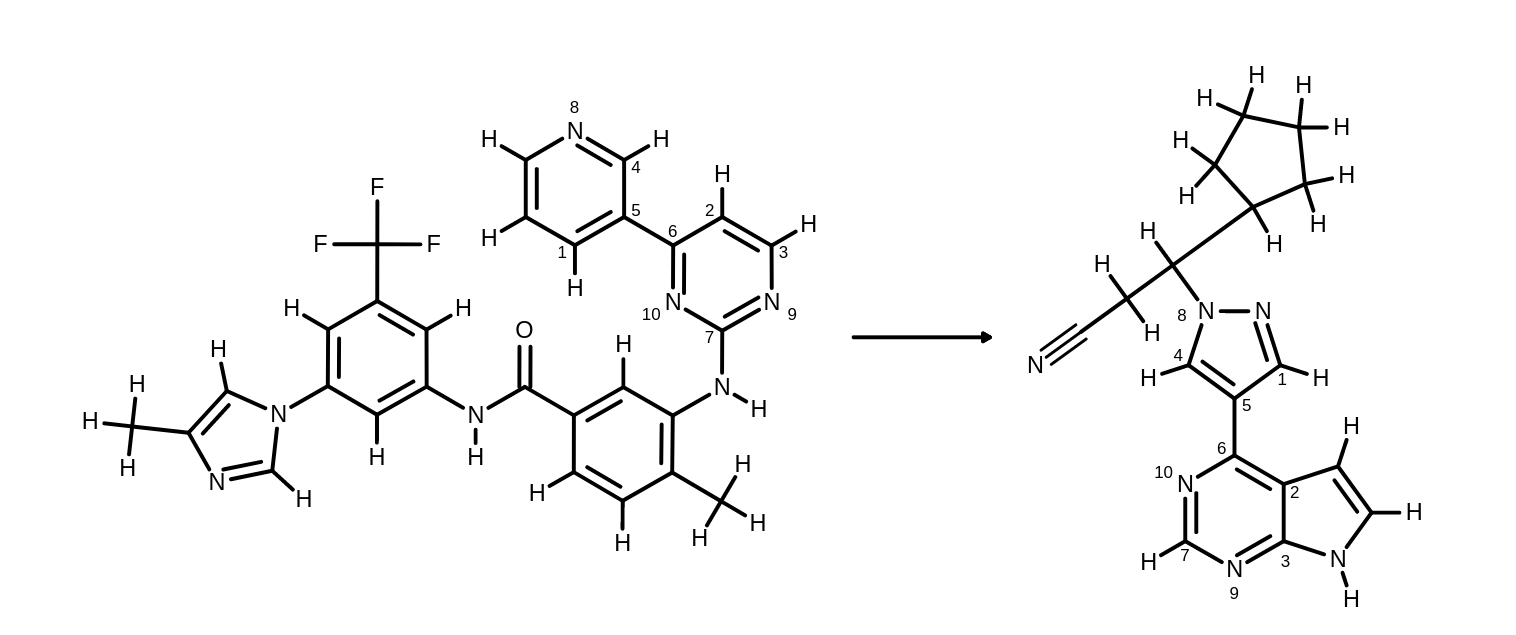
\includegraphics[width=1.0\textwidth]{kinase_map_bad.png}
    \caption{This map between kinase inhibitors may contain more atoms than another, but as it is partially breaking a ring, energies after the proposal are often highly unfavorable}
    \label{fig:bad_kinase_map}
\end{figure}
%
In Figure~\ref{fig:bad_kinase_map}, we see an example of the MCSS algorithm maximizing the overlap between two molecules in terms of the atom map.
%
However, it may be naive to attempt this, as the dimension-matching component of the algorithm will now have to complete the ring, and the annealing will have to gradually introduce part of the ring.
%
In this instance, the random choice of atom maps would be helpful, as the algorithm would occasionally not choose the ring-breaking map.
%
An attractive alternative to randomly choosing an atom map is to simply filter out maps that partially map rings.
%
While the toolkit that I used for this project unfortunately did not provide this as an option, it is possible to simply eliminate the maps that break rings.
%
The algorithm for determining whether rings are broken is as follows, with a return value of True signifying that rings are broken:
%
\begin{itemize}
    \item For a pair of molecules $(k, k')$, enumerate the cycle basis of both molecular graphs~\cite{paton1969algorithm}
    \item For each bond in a cycle of molecular graph $k$, check that it is in graph $k'$, if any are not, return True
    \item If all bonds in cycles of $k$ are also in $k'$, return False
\end{itemize}
%
This algorithm checks that rings are not created or destroyed, and is done using the NetworkX toolkit~\cite{Hagberg2008}.
%
However, building an entire ring is not infeasible, and so the algorithm could be modified to check that if a ring is created or broken, an entire ring is created or broken.
%
\subsection{An exploration of the effect of various atom mapping options on acceptance probability}
%
As an interesting exploration, I measured the empirical effect of different atom mappings on the variance of the instantaneous acceptance probabilities between various substituted benzene molecules as shown in Figure~\ref{fig:substituded_benzene_maps}.
%
\begin{figure}
    \centering
    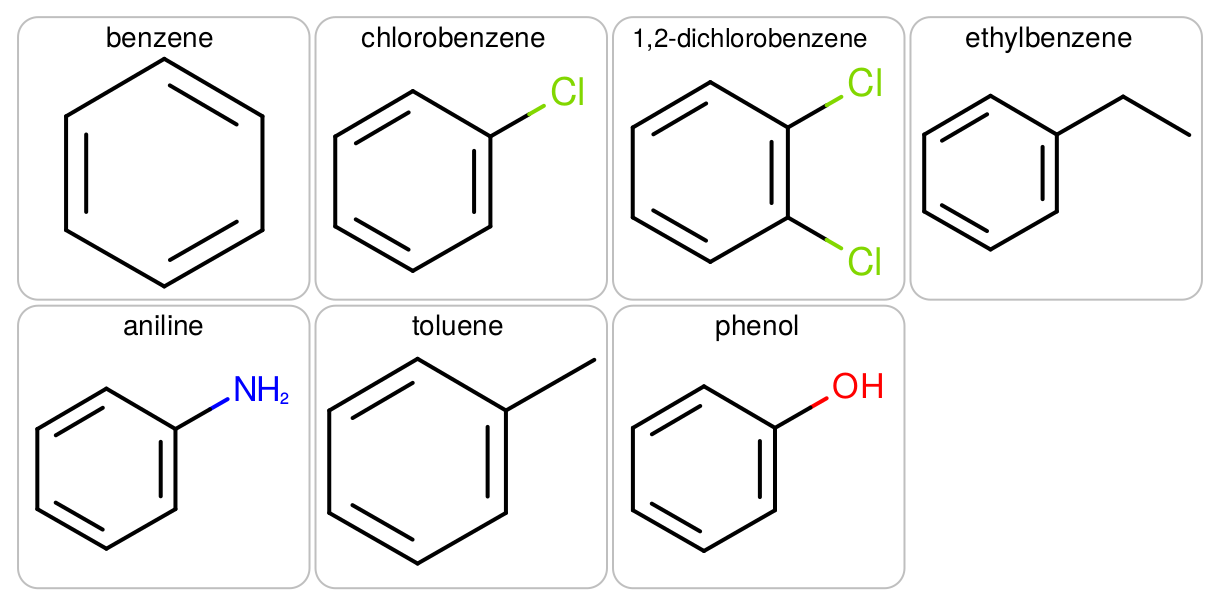
\includegraphics[width=0.5\textwidth]{mol_atom_map.png}
    \caption{The set of trial molecules used for empirical exploration of atom map criteria. This set was used to demonstrate because it contains very similar cores, but different substituents that might affect the performance of atom maps.
    }
    \label{fig:substituded_benzene_maps}
\end{figure}
%
In this experiment, I ran the molecules at a timestep of 1 femtosecond for 1 nanosecond at 300 Kelvin in vacuum, taking a snapshot of the trajectory every picosecond.
%
For each other molecule in the set, I attempted 100 reversible jump proposals under each atom matching scheme, starting from a configuration randomly drawn from the equilibrium cache of the starting molecule.
%
As is readily apparent from Figure~\ref{fig:benz_chlorobenz_different_maps}, the choice of map can have a significant effect on the quality of the proposal.
%
\begin{figure}
    \centering
    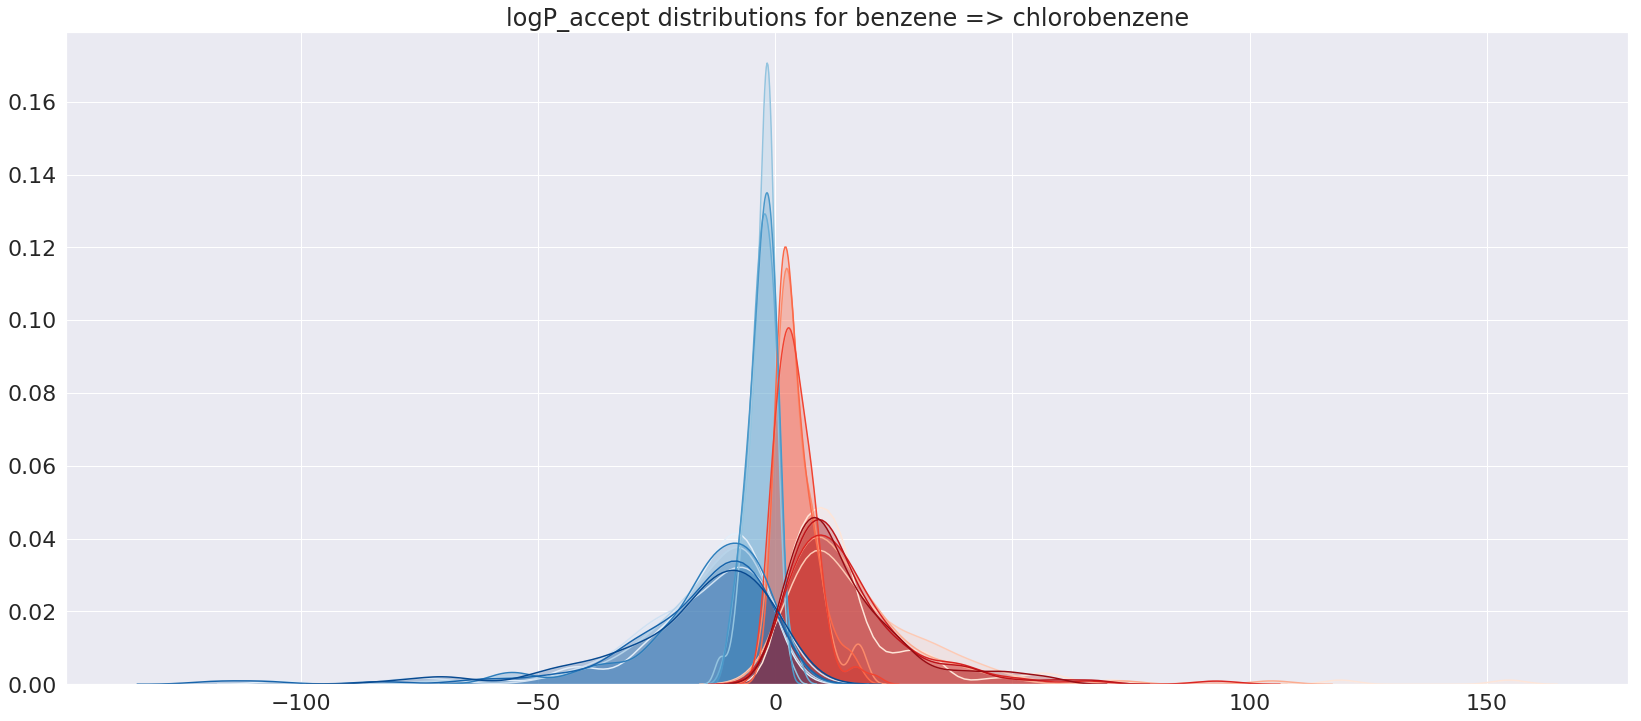
\includegraphics[width=\textwidth]{benzene_chlorobenzene_maps.png}
    \caption{Forward (blue) and negative reverse (red) log acceptance probability distributions for benzene to chlorobenzene in vacuum under different mapping schemes. Here, it is clearly visible that the choice of mapping scheme has a profound effect on the ultimate quality of the proposal.}
    \label{fig:benz_chlorobenz_different_maps}
\end{figure}
%
However, for some other pairs, the choice of map does not appear as important.
%
For example, in Figure~\ref{fig:toluene_phenol_different_maps}, the various maps produce distributions of acceptance probabilities that cluster around the the same region.
%
As such, it is an area of active investigation to determine how to map atoms in a way that maximizes the efficiency of the computation.
%
\begin{figure}
    \centering
    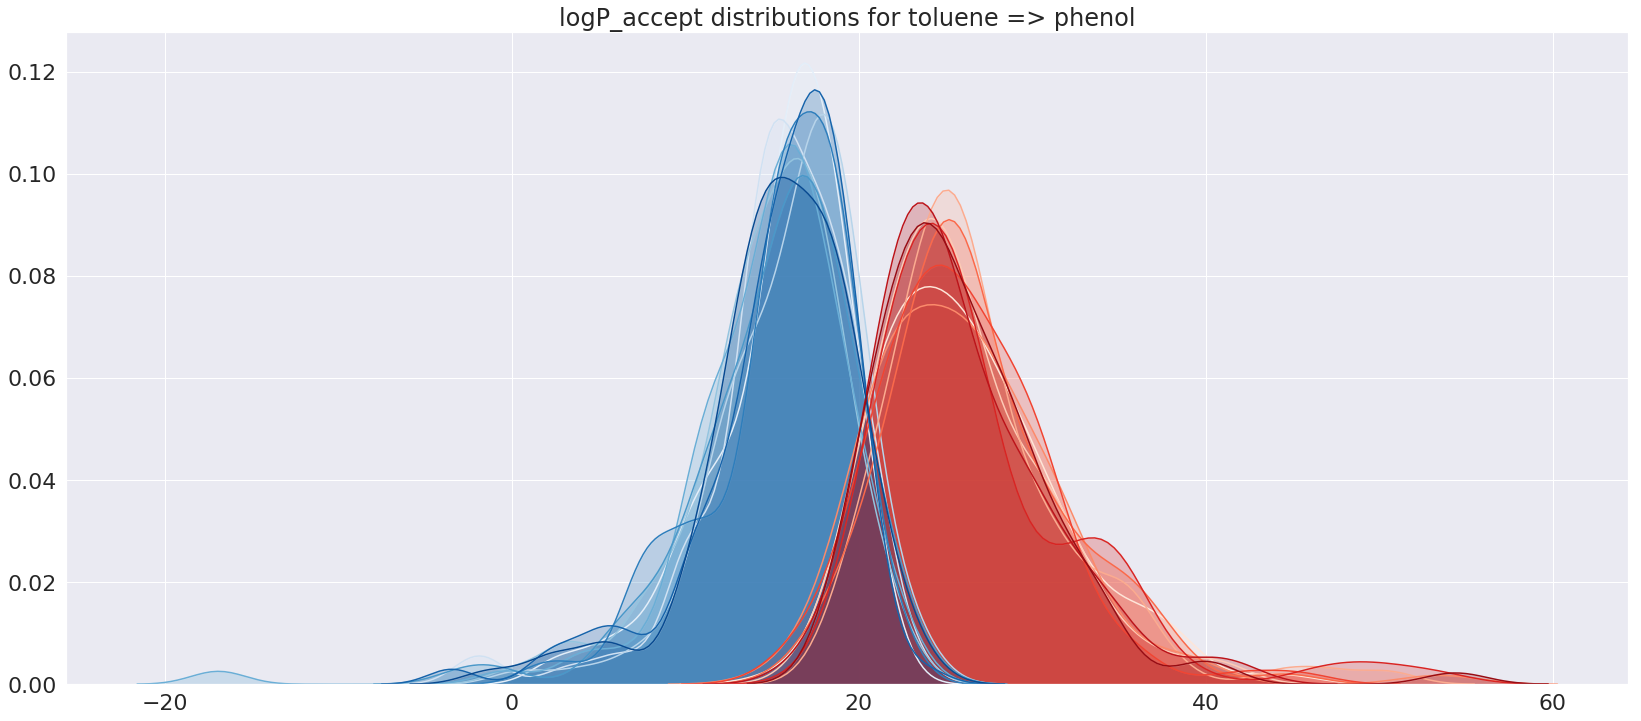
\includegraphics[width=\textwidth]{toluene_phenol_maps.png}
    \caption{Forward (blue) and negative reverse (red) log acceptance probability distributions for toluene to phenol in vacuum under different mapping schemes. Here, the choice of the mapping scheme does not seem to have as significant of an impact on the quality of the proposal.}
    \label{fig:toluene_phenol_different_maps}
\end{figure}
%
It is clearly of interest in practical applications to understand what the ideal atom mapping criterion for explicit solvent is, and whether this differs substantially from the criteria chosen in vacuum.
%
\section{Future work}
%
\subsection{Atom map learning}
For OpenEye MCSS, there are multiple atom map options.
%
For instance, the user can choose to have the MCSS algorithm match atoms based on aromaticity, element, number of heavy bond partners, and more.
%
In principle, these discrete choices can be enumerated and searched to find near-optimal combinations
%
This does leave open the question of what to use as the objective.
%
In principle, the variance of the acceptance probability is ideal, though it may be difficult to estimate.
%
Alternatively, one could try to find the set of discrete hyperparameters that maximize the average acceptance probability, which is straightforward to compute.
%
This does, however, leave the issue that a set of atom mapping parameters ideal for one set of molecules may not be performant for another.
%
\subsubsection{Treat atom mapping as a Reinforcement Learning problem}
%
As a result, one could imagine treating the atom mapping as a reinforcement learning problem, wherein an agent must select a set of parameters given the transformation at hand~\cite{Sutton1988, Watkins1992}.
%
In this way, one might hope that the algorithm could learn general rules that would be valid across many different sets of molecules.
%
One advantage of this approach is that, under certain conditions~\cite{Andrieu2005, Andrieu2007, Andrieu2008}, one could potentially design an adaptive MCMC algorithm that performs this learning as the calculation proceeds.
%
This would potentially allow the user to avoid a costly pre-optimization (or the use of suboptimal parameters derived from a reference set).
%
\subsubsection{Atom mapping with neural network}
%
Finally, one might also simply leave the atom mapping choice to a neural network, leaving open the possibility to efficiently learn a function mapping from transformations (or even environments) to atom maps.
%
Although the map itself is discrete, other sophisticated differentiable neural architectures such as the differentiable Forth interpreter~\cite{bosnjak17} were able to overcome this.
%
\subsection{Relieving the restriction to a finite set of chemicals}
%
Ideally, the simulation would not be limited to a prespecified set of chemical states.
%
Rather, one could imagine applying synthetic transformation rules to generate new, feasible chemicals.
%
This has the advantage of resulting in chemical matter that is more likely to be feasible to synthesize (or at least more likely to be able to convince a chemist to try).
%
Alternatively, one could imagine using an RNN such as in \cite{Gupta2017}, where a neural network might learn to generate new chemicals.
%
In this way, we might not only adaptively solve the issue of which chemical states are "neighboring," but also push toward synthetic novelty in a way that humans have not been able to.
%
Although there are challenges in this part of the algorithm, many of the challenges for expanding beyond a fixed set of chemical species lie in the weight adaptation algorithm, discussed later.
%
The development of this algorithm opens up new avenues for exploration, as well as new avenues for multidisciplinary collaboration with other fields.